\documentclass[1p]{elsarticle_modified}
%\bibliographystyle{elsarticle-num}

%\usepackage[colorlinks]{hyperref}
%\usepackage{abbrmath_seonhwa} %\Abb, \Ascr, \Acal ,\Abf, \Afrak
\usepackage{amsfonts}
\usepackage{amssymb}
\usepackage{amsmath}
\usepackage{amsthm}
\usepackage{scalefnt}
\usepackage{amsbsy}
\usepackage{kotex}
\usepackage{caption}
\usepackage{subfig}
\usepackage{color}
\usepackage{graphicx}
\usepackage{xcolor} %% white, black, red, green, blue, cyan, magenta, yellow
\usepackage{float}
\usepackage{setspace}
\usepackage{hyperref}

\usepackage{tikz}
\usetikzlibrary{arrows}

\usepackage{multirow}
\usepackage{array} % fixed length table
\usepackage{hhline}

%%%%%%%%%%%%%%%%%%%%%
\makeatletter
\renewcommand*\env@matrix[1][\arraystretch]{%
	\edef\arraystretch{#1}%
	\hskip -\arraycolsep
	\let\@ifnextchar\new@ifnextchar
	\array{*\c@MaxMatrixCols c}}
\makeatother %https://tex.stackexchange.com/questions/14071/how-can-i-increase-the-line-spacing-in-a-matrix
%%%%%%%%%%%%%%%

\usepackage[normalem]{ulem}

\newcommand{\msout}[1]{\ifmmode\text{\sout{\ensuremath{#1}}}\else\sout{#1}\fi}
%SOURCE: \msout is \stkout macro in https://tex.stackexchange.com/questions/20609/strikeout-in-math-mode

\newcommand{\cancel}[1]{
	\ifmmode
	{\color{red}\msout{#1}}
	\else
	{\color{red}\sout{#1}}
	\fi
}

\newcommand{\add}[1]{
	{\color{blue}\uwave{#1}}
}

\newcommand{\replace}[2]{
	\ifmmode
	{\color{red}\msout{#1}}{\color{blue}\uwave{#2}}
	\else
	{\color{red}\sout{#1}}{\color{blue}\uwave{#2}}
	\fi
}

\newcommand{\Sol}{\mathcal{S}} %segment
\newcommand{\D}{D} %diagram
\newcommand{\A}{\mathcal{A}} %arc


%%%%%%%%%%%%%%%%%%%%%%%%%%%%%5 test

\def\sl{\operatorname{\textup{SL}}(2,\Cbb)}
\def\psl{\operatorname{\textup{PSL}}(2,\Cbb)}
\def\quan{\mkern 1mu \triangleright \mkern 1mu}

\theoremstyle{definition}
\newtheorem{thm}{Theorem}[section]
\newtheorem{prop}[thm]{Proposition}
\newtheorem{lem}[thm]{Lemma}
\newtheorem{ques}[thm]{Question}
\newtheorem{cor}[thm]{Corollary}
\newtheorem{defn}[thm]{Definition}
\newtheorem{exam}[thm]{Example}
\newtheorem{rmk}[thm]{Remark}
\newtheorem{alg}[thm]{Algorithm}

\newcommand{\I}{\sqrt{-1}}
\begin{document}

%\begin{frontmatter}
%
%\title{Boundary parabolic representations of knots up to 8 crossings}
%
%%% Group authors per affiliation:
%\author{Yunhi Cho} 
%\address{Department of Mathematics, University of Seoul, Seoul, Korea}
%\ead{yhcho@uos.ac.kr}
%
%
%\author{Seonhwa Kim} %\fnref{s_kim}}
%\address{Center for Geometry and Physics, Institute for Basic Science, Pohang, 37673, Korea}
%\ead{ryeona17@ibs.re.kr}
%
%\author{Hyuk Kim}
%\address{Department of Mathematical Sciences, Seoul National University, Seoul 08826, Korea}
%\ead{hyukkim@snu.ac.kr}
%
%\author{Seokbeom Yoon}
%\address{Department of Mathematical Sciences, Seoul National University, Seoul, 08826,  Korea}
%\ead{sbyoon15@snu.ac.kr}
%
%\begin{abstract}
%We find all boundary parabolic representation of knots up to 8 crossings.
%
%\end{abstract}
%\begin{keyword}
%    \MSC[2010] 57M25 
%\end{keyword}
%
%\end{frontmatter}

%\linenumbers
%\tableofcontents
%
\newcommand\colored[1]{\textcolor{white}{\rule[-0.35ex]{0.8em}{1.4ex}}\kern-0.8em\color{red} #1}%
%\newcommand\colored[1]{\textcolor{white}{ #1}\kern-2.17ex	\textcolor{white}{ #1}\kern-1.81ex	\textcolor{white}{ #1}\kern-2.15ex\color{red}#1	}

{\Large $\underline{11a_{16}~(K11a_{16})}$}

\setlength{\tabcolsep}{10pt}
\renewcommand{\arraystretch}{1.6}
\vspace{1cm}\begin{tabular}{m{100pt}>{\centering\arraybackslash}m{274pt}}
\multirow{5}{120pt}{
	\centering
	\includegraphics[width=112pt]{../../../GIT/diagram.site/Diagrams/png/265_11a_16.png}\\
\ \ \ A knot diagram\footnotemark}&
\allowdisplaybreaks
\textbf{Linearized knot diagam} \\
\cline{2-2}
 &
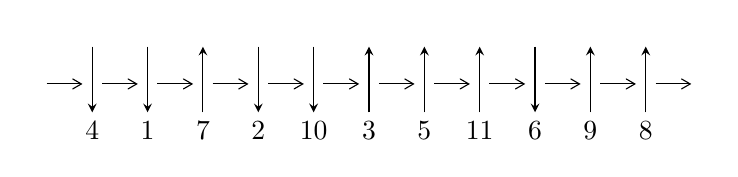
\begin{tikzpicture}[x=20pt, y=17pt]
	% nodes
	\node (C0) at (0, 0) {};
	\node (C1) at (1, 0) {};
	\node (C1U) at (1, +1) {};
	\node (C1D) at (1, -1) {4};

	\node (C2) at (2, 0) {};
	\node (C2U) at (2, +1) {};
	\node (C2D) at (2, -1) {1};

	\node (C3) at (3, 0) {};
	\node (C3U) at (3, +1) {};
	\node (C3D) at (3, -1) {7};

	\node (C4) at (4, 0) {};
	\node (C4U) at (4, +1) {};
	\node (C4D) at (4, -1) {2};

	\node (C5) at (5, 0) {};
	\node (C5U) at (5, +1) {};
	\node (C5D) at (5, -1) {10};

	\node (C6) at (6, 0) {};
	\node (C6U) at (6, +1) {};
	\node (C6D) at (6, -1) {3};

	\node (C7) at (7, 0) {};
	\node (C7U) at (7, +1) {};
	\node (C7D) at (7, -1) {5};

	\node (C8) at (8, 0) {};
	\node (C8U) at (8, +1) {};
	\node (C8D) at (8, -1) {11};

	\node (C9) at (9, 0) {};
	\node (C9U) at (9, +1) {};
	\node (C9D) at (9, -1) {6};

	\node (C10) at (10, 0) {};
	\node (C10U) at (10, +1) {};
	\node (C10D) at (10, -1) {9};

	\node (C11) at (11, 0) {};
	\node (C11U) at (11, +1) {};
	\node (C11D) at (11, -1) {8};
	\node (C12) at (12, 0) {};

	% arrows
	\draw[->,>={angle 60}]
	(C0) edge (C1) (C1) edge (C2) (C2) edge (C3) (C3) edge (C4) (C4) edge (C5) (C5) edge (C6) (C6) edge (C7) (C7) edge (C8) (C8) edge (C9) (C9) edge (C10) (C10) edge (C11) (C11) edge (C12) ;	\draw[->,>=stealth]
	(C1U) edge (C1D) (C2U) edge (C2D) (C3D) edge (C3U) (C4U) edge (C4D) (C5U) edge (C5D) (C6D) edge (C6U) (C7D) edge (C7U) (C8D) edge (C8U) (C9U) edge (C9D) (C10D) edge (C10U) (C11D) edge (C11U) ;
	\end{tikzpicture} \\
\hhline{~~} \\& 
\textbf{Solving Sequence} \\ \cline{2-2} 
 &
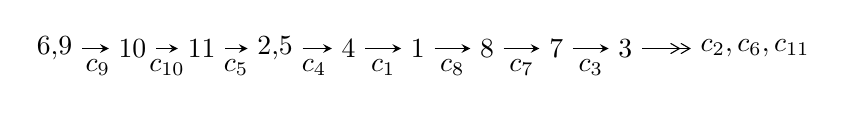
\begin{tikzpicture}[x=25pt, y=7pt]
	% node
	\node (A0) at (-1/8, 0) {6,9};
	\node (A1) at (1, 0) {10};
	\node (A2) at (2, 0) {11};
	\node (A3) at (49/16, 0) {2,5};
	\node (A4) at (33/8, 0) {4};
	\node (A5) at (41/8, 0) {1};
	\node (A6) at (49/8, 0) {8};
	\node (A7) at (57/8, 0) {7};
	\node (A8) at (65/8, 0) {3};
	\node (C1) at (1/2, -1) {$c_{9}$};
	\node (C2) at (3/2, -1) {$c_{10}$};
	\node (C3) at (5/2, -1) {$c_{5}$};
	\node (C4) at (29/8, -1) {$c_{4}$};
	\node (C5) at (37/8, -1) {$c_{1}$};
	\node (C6) at (45/8, -1) {$c_{8}$};
	\node (C7) at (53/8, -1) {$c_{7}$};
	\node (C8) at (61/8, -1) {$c_{3}$};
	\node (A9) at (10, 0) {$c_{2},c_{6},c_{11}$};

	% edge
	\draw[->,>=stealth]	
	(A0) edge (A1) (A1) edge (A2) (A2) edge (A3) (A3) edge (A4) (A4) edge (A5) (A5) edge (A6) (A6) edge (A7) (A7) edge (A8) ;
	\draw[->>,>={angle 60}]	
	(A8) edge (A9);
\end{tikzpicture} \\ 

\end{tabular} \\

\footnotetext{
The image of knot diagram is generated by the software ``\textbf{Draw programme}" developed by Andrew Bartholomew(\url{http://www.layer8.co.uk/maths/draw/index.htm\#Running-draw}), where we modified some parts for our purpose(\url{https://github.com/CATsTAILs/LinksPainter}).
}\phantom \\ \newline 
\centering \textbf{Ideals for irreducible components\footnotemark of $X_{\text{par}}$} 
 
\begin{align*}
I^u_{1}&=\langle 
u^{53}+u^{52}+\cdots+5 u^4+b,\;- u^{33}-4 u^{31}+\cdots+a- u,\;u^{56}+2 u^{55}+\cdots+2 u^2+1\rangle \\
I^u_{2}&=\langle 
u^2+b,\;a+u,\;u^4- u^3+u^2+1\rangle \\
\\
\end{align*}
\raggedright * 2 irreducible components of $\dim_{\mathbb{C}}=0$, with total 60 representations.\\
\footnotetext{All coefficients of polynomials are rational numbers. But the coefficients are sometimes approximated in decimal forms when there is not enough margin.}
\newpage
\renewcommand{\arraystretch}{1}
\centering \section*{I. $I^u_{1}= \langle u^{53}+u^{52}+\cdots+5 u^4+b,\;- u^{33}-4 u^{31}+\cdots+a- u,\;u^{56}+2 u^{55}+\cdots+2 u^2+1 \rangle$}
\flushleft \textbf{(i) Arc colorings}\\
\begin{tabular}{m{7pt} m{180pt} m{7pt} m{180pt} }
\flushright $a_{6}=$&$\begin{pmatrix}0\\u\end{pmatrix}$ \\
\flushright $a_{9}=$&$\begin{pmatrix}1\\0\end{pmatrix}$ \\
\flushright $a_{10}=$&$\begin{pmatrix}1\\u^2\end{pmatrix}$ \\
\flushright $a_{11}=$&$\begin{pmatrix}u^2+1\\u^2\end{pmatrix}$ \\
\flushright $a_{2}=$&$\begin{pmatrix}u^{33}+4 u^{31}+\cdots+8 u^3+u\\- u^{53}- u^{52}+\cdots+5 u^5-5 u^4\end{pmatrix}$ \\
\flushright $a_{5}=$&$\begin{pmatrix}u\\u^3+u\end{pmatrix}$ \\
\flushright $a_{4}=$&$\begin{pmatrix}u^{55}+u^{54}+\cdots+2 u^2+1\\u^{55}+2 u^{54}+\cdots+3 u^2+1\end{pmatrix}$ \\
\flushright $a_{1}=$&$\begin{pmatrix}u^6+u^4+2 u^2+1\\u^6+u^2\end{pmatrix}$ \\
\flushright $a_{8}=$&$\begin{pmatrix}u^4+u^2+1\\u^4\end{pmatrix}$ \\
\flushright $a_{7}=$&$\begin{pmatrix}u^8+u^6+3 u^4+2 u^2+1\\u^{10}+2 u^8+3 u^6+4 u^4+u^2\end{pmatrix}$ \\
\flushright $a_{3}=$&$\begin{pmatrix}- u^{55}- u^{54}+\cdots-9 u^5-5 u^3\\- u^{55}-2 u^{54}+\cdots+u-1\end{pmatrix}$\\ \flushright $a_{3}=$&$\begin{pmatrix}- u^{55}- u^{54}+\cdots-9 u^5-5 u^3\\- u^{55}-2 u^{54}+\cdots+u-1\end{pmatrix}$\\&\end{tabular}
\flushleft \textbf{(ii) Obstruction class $= -1$}\\~\\
\flushleft \textbf{(iii) Cusp Shapes $= -4 u^{55}-25 u^{53}+\cdots-11 u+3$}\\~\\
\newpage\renewcommand{\arraystretch}{1}
\flushleft \textbf{(iv) u-Polynomials at the component}\newline \\
\begin{tabular}{m{50pt}|m{274pt}}
Crossings & \hspace{64pt}u-Polynomials at each crossing \\
\hline $$\begin{aligned}c_{1},c_{4}\end{aligned}$$&$\begin{aligned}
&u^{56}-5 u^{55}+\cdots-2 u+1
\end{aligned}$\\
\hline $$\begin{aligned}c_{2}\end{aligned}$$&$\begin{aligned}
&u^{56}+27 u^{55}+\cdots-30 u+1
\end{aligned}$\\
\hline $$\begin{aligned}c_{3},c_{6}\end{aligned}$$&$\begin{aligned}
&u^{56}- u^{55}+\cdots-56 u+16
\end{aligned}$\\
\hline $$\begin{aligned}c_{5},c_{9}\end{aligned}$$&$\begin{aligned}
&u^{56}+2 u^{55}+\cdots+2 u^2+1
\end{aligned}$\\
\hline $$\begin{aligned}c_{7}\end{aligned}$$&$\begin{aligned}
&u^{56}+2 u^{55}+\cdots-140 u+200
\end{aligned}$\\
\hline $$\begin{aligned}c_{8},c_{10},c_{11}\end{aligned}$$&$\begin{aligned}
&u^{56}-14 u^{55}+\cdots-4 u+1
\end{aligned}$\\
\hline
\end{tabular}\\~\\
\newpage\renewcommand{\arraystretch}{1}
\flushleft \textbf{(v) Riley Polynomials at the component}\newline \\
\begin{tabular}{m{50pt}|m{274pt}}
Crossings & \hspace{64pt}Riley Polynomials at each crossing \\
\hline $$\begin{aligned}c_{1},c_{4}\end{aligned}$$&$\begin{aligned}
&y^{56}-27 y^{55}+\cdots+30 y+1
\end{aligned}$\\
\hline $$\begin{aligned}c_{2}\end{aligned}$$&$\begin{aligned}
&y^{56}+9 y^{55}+\cdots-730 y+1
\end{aligned}$\\
\hline $$\begin{aligned}c_{3},c_{6}\end{aligned}$$&$\begin{aligned}
&y^{56}-27 y^{55}+\cdots-2624 y+256
\end{aligned}$\\
\hline $$\begin{aligned}c_{5},c_{9}\end{aligned}$$&$\begin{aligned}
&y^{56}+14 y^{55}+\cdots+4 y+1
\end{aligned}$\\
\hline $$\begin{aligned}c_{7}\end{aligned}$$&$\begin{aligned}
&y^{56}-2 y^{55}+\cdots+62800 y+40000
\end{aligned}$\\
\hline $$\begin{aligned}c_{8},c_{10},c_{11}\end{aligned}$$&$\begin{aligned}
&y^{56}+58 y^{55}+\cdots+28 y+1
\end{aligned}$\\
\hline
\end{tabular}\\~\\
\newpage\flushleft \textbf{(vi) Complex Volumes and Cusp Shapes}
$$\begin{array}{c|c|c}  
\text{Solutions to }I^u_{1}& \I (\text{vol} + \sqrt{-1}CS) & \text{Cusp shape}\\
 \hline 
\begin{aligned}
u &= -0.607473 + 0.783881 I \\
a &= -0.002331 - 0.683957 I \\
b &= -0.598837 + 0.456874 I\end{aligned}
 & -0.0338562 + 0.1100990 I & \phantom{-}1.75833 - 0.05075 I \\ \hline\begin{aligned}
u &= -0.607473 - 0.783881 I \\
a &= -0.002331 + 0.683957 I \\
b &= -0.598837 - 0.456874 I\end{aligned}
 & -0.0338562 - 0.1100990 I & \phantom{-}1.75833 + 0.05075 I \\ \hline\begin{aligned}
u &= \phantom{-}0.197770 + 0.968662 I \\
a &= -1.174190 + 0.456988 I \\
b &= -1.195730 - 0.002117 I\end{aligned}
 & \phantom{-}5.73525 - 1.07098 I & \phantom{-}8.88776 + 3.00045 I \\ \hline\begin{aligned}
u &= \phantom{-}0.197770 - 0.968662 I \\
a &= -1.174190 - 0.456988 I \\
b &= -1.195730 + 0.002117 I\end{aligned}
 & \phantom{-}5.73525 + 1.07098 I & \phantom{-}8.88776 - 3.00045 I \\ \hline\begin{aligned}
u &= \phantom{-}0.134977 + 0.977631 I \\
a &= \phantom{-}1.153010 + 0.242929 I \\
b &= \phantom{-}0.51633 + 1.44724 I\end{aligned}
 & \phantom{-}4.33416 + 4.34991 I & \phantom{-}6.75272 - 2.91610 I \\ \hline\begin{aligned}
u &= \phantom{-}0.134977 - 0.977631 I \\
a &= \phantom{-}1.153010 - 0.242929 I \\
b &= \phantom{-}0.51633 - 1.44724 I\end{aligned}
 & \phantom{-}4.33416 - 4.34991 I & \phantom{-}6.75272 + 2.91610 I \\ \hline\begin{aligned}
u &= -0.336798 + 0.920797 I \\
a &= -1.96894 - 0.80256 I \\
b &= -1.82104 + 0.28973 I\end{aligned}
 & \phantom{-}0.23022 + 4.40037 I & \phantom{-}2.37312 - 7.37153 I \\ \hline\begin{aligned}
u &= -0.336798 - 0.920797 I \\
a &= -1.96894 + 0.80256 I \\
b &= -1.82104 - 0.28973 I\end{aligned}
 & \phantom{-}0.23022 - 4.40037 I & \phantom{-}2.37312 + 7.37153 I \\ \hline\begin{aligned}
u &= \phantom{-}0.332306 + 0.976151 I \\
a &= \phantom{-}0.935169 + 0.500138 I \\
b &= \phantom{-}0.46182 + 1.35862 I\end{aligned}
 & \phantom{-}4.96310 - 4.62849 I & \phantom{-}7.03327 + 5.15784 I \\ \hline\begin{aligned}
u &= \phantom{-}0.332306 - 0.976151 I \\
a &= \phantom{-}0.935169 - 0.500138 I \\
b &= \phantom{-}0.46182 - 1.35862 I\end{aligned}
 & \phantom{-}4.96310 + 4.62849 I & \phantom{-}7.03327 - 5.15784 I\\
 \hline 
 \end{array}$$\newpage$$\begin{array}{c|c|c}  
\text{Solutions to }I^u_{1}& \I (\text{vol} + \sqrt{-1}CS) & \text{Cusp shape}\\
 \hline 
\begin{aligned}
u &= \phantom{-}0.374376 + 0.988459 I \\
a &= -1.88884 + 0.26158 I \\
b &= -1.43993 - 0.58440 I\end{aligned}
 & \phantom{-}2.95830 - 10.14670 I & \phantom{-}3.62258 + 9.49522 I \\ \hline\begin{aligned}
u &= \phantom{-}0.374376 - 0.988459 I \\
a &= -1.88884 - 0.26158 I \\
b &= -1.43993 + 0.58440 I\end{aligned}
 & \phantom{-}2.95830 + 10.14670 I & \phantom{-}3.62258 - 9.49522 I \\ \hline\begin{aligned}
u &= \phantom{-}0.316154 + 0.867764 I \\
a &= \phantom{-}0.481267 + 0.459650 I \\
b &= \phantom{-}0.272900 - 0.852680 I\end{aligned}
 & -0.79958 - 2.18057 I & \phantom{-}4.75108 + 6.92304 I \\ \hline\begin{aligned}
u &= \phantom{-}0.316154 - 0.867764 I \\
a &= \phantom{-}0.481267 - 0.459650 I \\
b &= \phantom{-}0.272900 + 0.852680 I\end{aligned}
 & -0.79958 + 2.18057 I & \phantom{-}4.75108 - 6.92304 I \\ \hline\begin{aligned}
u &= -0.698952 + 0.836112 I \\
a &= -0.335932 - 0.700898 I \\
b &= -1.068380 + 0.795592 I\end{aligned}
 & -0.0629739 + 0.1237040 I & \phantom{-}2.10228 + 0. I\phantom{ +0.000000I} \\ \hline\begin{aligned}
u &= -0.698952 - 0.836112 I \\
a &= -0.335932 + 0.700898 I \\
b &= -1.068380 - 0.795592 I\end{aligned}
 & -0.0629739 - 0.1237040 I & \phantom{-}2.10228 + 0. I\phantom{ +0.000000I} \\ \hline\begin{aligned}
u &= -0.226190 + 0.873692 I \\
a &= \phantom{-}1.35876 - 0.68991 I \\
b &= \phantom{-}0.37876 - 1.64298 I\end{aligned}
 & \phantom{-}0.899368 + 0.464839 I & \phantom{-}4.81093 - 1.16758 I \\ \hline\begin{aligned}
u &= -0.226190 - 0.873692 I \\
a &= \phantom{-}1.35876 + 0.68991 I \\
b &= \phantom{-}0.37876 + 1.64298 I\end{aligned}
 & \phantom{-}0.899368 - 0.464839 I & \phantom{-}4.81093 + 1.16758 I \\ \hline\begin{aligned}
u &= -0.642289 + 0.536924 I \\
a &= -0.272696 - 0.336147 I \\
b &= \phantom{-}0.767444 + 0.080263 I\end{aligned}
 & -0.84678 + 4.37124 I & -1.57903 - 6.34104 I \\ \hline\begin{aligned}
u &= -0.642289 - 0.536924 I \\
a &= -0.272696 + 0.336147 I \\
b &= \phantom{-}0.767444 - 0.080263 I\end{aligned}
 & -0.84678 - 4.37124 I & -1.57903 + 6.34104 I\\
 \hline 
 \end{array}$$\newpage$$\begin{array}{c|c|c}  
\text{Solutions to }I^u_{1}& \I (\text{vol} + \sqrt{-1}CS) & \text{Cusp shape}\\
 \hline 
\begin{aligned}
u &= -0.739754 + 0.929885 I \\
a &= \phantom{-}0.982797 + 0.454600 I \\
b &= \phantom{-}2.17782 - 0.94804 I\end{aligned}
 & \phantom{-}0.25420 + 5.44548 I & \phantom{-0.000000 } 0 \\ \hline\begin{aligned}
u &= -0.739754 - 0.929885 I \\
a &= \phantom{-}0.982797 - 0.454600 I \\
b &= \phantom{-}2.17782 + 0.94804 I\end{aligned}
 & \phantom{-}0.25420 - 5.44548 I & \phantom{-0.000000 } 0 \\ \hline\begin{aligned}
u &= -0.863121 + 0.817193 I \\
a &= -0.319367 + 0.570837 I \\
b &= \phantom{-}1.166920 + 0.719296 I\end{aligned}
 & -2.72661 - 2.68562 I & \phantom{-0.000000 } 0 \\ \hline\begin{aligned}
u &= -0.863121 - 0.817193 I \\
a &= -0.319367 - 0.570837 I \\
b &= \phantom{-}1.166920 - 0.719296 I\end{aligned}
 & -2.72661 + 2.68562 I & \phantom{-0.000000 } 0 \\ \hline\begin{aligned}
u &= \phantom{-}0.826658 + 0.867184 I \\
a &= -0.143454 - 0.975542 I \\
b &= \phantom{-}1.83509 - 1.02941 I\end{aligned}
 & -5.44180 - 2.46519 I & \phantom{-0.000000 } 0 \\ \hline\begin{aligned}
u &= \phantom{-}0.826658 - 0.867184 I \\
a &= -0.143454 + 0.975542 I \\
b &= \phantom{-}1.83509 + 1.02941 I\end{aligned}
 & -5.44180 + 2.46519 I & \phantom{-0.000000 } 0 \\ \hline\begin{aligned}
u &= \phantom{-}0.857567 + 0.839377 I \\
a &= -0.74269 + 2.21222 I \\
b &= -3.62706 + 0.28882 I\end{aligned}
 & -7.29705 + 1.90076 I & \phantom{-0.000000 } 0 \\ \hline\begin{aligned}
u &= \phantom{-}0.857567 - 0.839377 I \\
a &= -0.74269 - 2.21222 I \\
b &= -3.62706 - 0.28882 I\end{aligned}
 & -7.29705 - 1.90076 I & \phantom{-0.000000 } 0 \\ \hline\begin{aligned}
u &= -0.849620 + 0.854105 I \\
a &= -0.792263 + 1.139890 I \\
b &= -0.00621 + 1.65871 I\end{aligned}
 & -8.01940 + 0.73257 I & \phantom{-0.000000 } 0 \\ \hline\begin{aligned}
u &= -0.849620 - 0.854105 I \\
a &= -0.792263 - 1.139890 I \\
b &= -0.00621 - 1.65871 I\end{aligned}
 & -8.01940 - 0.73257 I & \phantom{-0.000000 } 0\\
 \hline 
 \end{array}$$\newpage$$\begin{array}{c|c|c}  
\text{Solutions to }I^u_{1}& \I (\text{vol} + \sqrt{-1}CS) & \text{Cusp shape}\\
 \hline 
\begin{aligned}
u &= -0.885456 + 0.821796 I \\
a &= -0.17654 - 2.19494 I \\
b &= -3.02543 - 1.15202 I\end{aligned}
 & -5.23615 - 8.13965 I & \phantom{-0.000000 } 0 \\ \hline\begin{aligned}
u &= -0.885456 - 0.821796 I \\
a &= -0.17654 + 2.19494 I \\
b &= -3.02543 + 1.15202 I\end{aligned}
 & -5.23615 + 8.13965 I & \phantom{-0.000000 } 0 \\ \hline\begin{aligned}
u &= \phantom{-}0.806000 + 0.927194 I \\
a &= -1.071000 - 0.159961 I \\
b &= -0.71417 - 2.31552 I\end{aligned}
 & -5.25339 - 3.63777 I & \phantom{-0.000000 } 0 \\ \hline\begin{aligned}
u &= \phantom{-}0.806000 - 0.927194 I \\
a &= -1.071000 + 0.159961 I \\
b &= -0.71417 + 2.31552 I\end{aligned}
 & -5.25339 + 3.63777 I & \phantom{-0.000000 } 0 \\ \hline\begin{aligned}
u &= -0.815993 + 0.946530 I \\
a &= -1.036900 + 0.852297 I \\
b &= -0.033804 + 1.372620 I\end{aligned}
 & -7.72972 + 5.47011 I & \phantom{-0.000000 } 0 \\ \hline\begin{aligned}
u &= -0.815993 - 0.946530 I \\
a &= -1.036900 - 0.852297 I \\
b &= -0.033804 - 1.372620 I\end{aligned}
 & -7.72972 - 5.47011 I & \phantom{-0.000000 } 0 \\ \hline\begin{aligned}
u &= \phantom{-}0.878810 + 0.896198 I \\
a &= -0.711275 - 0.954669 I \\
b &= \phantom{-}0.07035 - 1.68065 I\end{aligned}
 & -8.57446 - 4.40882 I & \phantom{-0.000000 } 0 \\ \hline\begin{aligned}
u &= \phantom{-}0.878810 - 0.896198 I \\
a &= -0.711275 + 0.954669 I \\
b &= \phantom{-}0.07035 + 1.68065 I\end{aligned}
 & -8.57446 + 4.40882 I & \phantom{-0.000000 } 0 \\ \hline\begin{aligned}
u &= \phantom{-}0.813621 + 0.959611 I \\
a &= \phantom{-}2.19976 - 0.71809 I \\
b &= \phantom{-}3.61245 + 2.54974 I\end{aligned}
 & -6.92091 - 8.11870 I & \phantom{-0.000000 } 0 \\ \hline\begin{aligned}
u &= \phantom{-}0.813621 - 0.959611 I \\
a &= \phantom{-}2.19976 + 0.71809 I \\
b &= \phantom{-}3.61245 - 2.54974 I\end{aligned}
 & -6.92091 + 8.11870 I & \phantom{-0.000000 } 0\\
 \hline 
 \end{array}$$\newpage$$\begin{array}{c|c|c}  
\text{Solutions to }I^u_{1}& \I (\text{vol} + \sqrt{-1}CS) & \text{Cusp shape}\\
 \hline 
\begin{aligned}
u &= -0.805941 + 0.974641 I \\
a &= -0.652089 + 0.274125 I \\
b &= -0.40013 + 1.87733 I\end{aligned}
 & -2.23567 + 8.89297 I & \phantom{-0.000000 } 0 \\ \hline\begin{aligned}
u &= -0.805941 - 0.974641 I \\
a &= -0.652089 - 0.274125 I \\
b &= -0.40013 - 1.87733 I\end{aligned}
 & -2.23567 - 8.89297 I & \phantom{-0.000000 } 0 \\ \hline\begin{aligned}
u &= \phantom{-}0.861222 + 0.936822 I \\
a &= -0.884065 - 0.792933 I \\
b &= \phantom{-}0.195344 - 1.380390 I\end{aligned}
 & -8.44550 - 2.02974 I & \phantom{-0.000000 } 0 \\ \hline\begin{aligned}
u &= \phantom{-}0.861222 - 0.936822 I \\
a &= -0.884065 + 0.792933 I \\
b &= \phantom{-}0.195344 + 1.380390 I\end{aligned}
 & -8.44550 + 2.02974 I & \phantom{-0.000000 } 0 \\ \hline\begin{aligned}
u &= -0.819387 + 0.983775 I \\
a &= \phantom{-}2.17573 + 0.14098 I \\
b &= \phantom{-}2.71437 - 3.01653 I\end{aligned}
 & -4.7257 + 14.4579 I & \phantom{-0.000000 } 0 \\ \hline\begin{aligned}
u &= -0.819387 - 0.983775 I \\
a &= \phantom{-}2.17573 - 0.14098 I \\
b &= \phantom{-}2.71437 + 3.01653 I\end{aligned}
 & -4.7257 - 14.4579 I & \phantom{-0.000000 } 0 \\ \hline\begin{aligned}
u &= -0.281383 + 0.637058 I \\
a &= \phantom{-}0.264556 - 0.604336 I \\
b &= -0.341113 - 0.409388 I\end{aligned}
 & \phantom{-}0.260433 + 1.109870 I & \phantom{-}3.40522 - 6.21684 I \\ \hline\begin{aligned}
u &= -0.281383 - 0.637058 I \\
a &= \phantom{-}0.264556 + 0.604336 I \\
b &= -0.341113 + 0.409388 I\end{aligned}
 & \phantom{-}0.260433 - 1.109870 I & \phantom{-}3.40522 + 6.21684 I \\ \hline\begin{aligned}
u &= \phantom{-}0.660025 + 0.212760 I \\
a &= \phantom{-}0.82341 - 1.92825 I \\
b &= \phantom{-}0.462433 - 1.144870 I\end{aligned}
 & \phantom{-}0.50522 + 6.42800 I & -1.79832 - 5.15907 I \\ \hline\begin{aligned}
u &= \phantom{-}0.660025 - 0.212760 I \\
a &= \phantom{-}0.82341 + 1.92825 I \\
b &= \phantom{-}0.462433 + 1.144870 I\end{aligned}
 & \phantom{-}0.50522 - 6.42800 I & -1.79832 + 5.15907 I\\
 \hline 
 \end{array}$$\newpage$$\begin{array}{c|c|c}  
\text{Solutions to }I^u_{1}& \I (\text{vol} + \sqrt{-1}CS) & \text{Cusp shape}\\
 \hline 
\begin{aligned}
u &= \phantom{-}0.605642 + 0.131913 I \\
a &= \phantom{-}0.88096 + 1.17599 I \\
b &= \phantom{-}0.032323 + 0.705281 I\end{aligned}
 & \phantom{-}2.38315 + 1.29675 I & \phantom{-}1.42442 - 0.64044 I \\ \hline\begin{aligned}
u &= \phantom{-}0.605642 - 0.131913 I \\
a &= \phantom{-}0.88096 - 1.17599 I \\
b &= \phantom{-}0.032323 - 0.705281 I\end{aligned}
 & \phantom{-}2.38315 - 1.29675 I & \phantom{-}1.42442 + 0.64044 I \\ \hline\begin{aligned}
u &= \phantom{-}0.384124 + 0.388656 I \\
a &= -0.517188 + 1.130980 I \\
b &= \phantom{-}0.805658 - 0.181951 I\end{aligned}
 & -2.27622 - 0.63522 I & -5.14216 - 1.49241 I \\ \hline\begin{aligned}
u &= \phantom{-}0.384124 - 0.388656 I \\
a &= -0.517188 - 1.130980 I \\
b &= \phantom{-}0.805658 + 0.181951 I\end{aligned}
 & -2.27622 + 0.63522 I & -5.14216 + 1.49241 I \\ \hline\begin{aligned}
u &= -0.476893 + 0.223440 I \\
a &= \phantom{-}1.43434 + 2.19416 I \\
b &= \phantom{-}0.801838 + 0.868626 I\end{aligned}
 & -1.82537 - 1.28944 I & -5.03333 + 1.67156 I \\ \hline\begin{aligned}
u &= -0.476893 - 0.223440 I \\
a &= \phantom{-}1.43434 - 2.19416 I \\
b &= \phantom{-}0.801838 - 0.868626 I\end{aligned}
 & -1.82537 + 1.28944 I & -5.03333 - 1.67156 I\\
 \hline 
 \end{array}$$\newpage\newpage\renewcommand{\arraystretch}{1}
\centering \section*{II. $I^u_{2}= \langle u^2+b,\;a+u,\;u^4- u^3+u^2+1 \rangle$}
\flushleft \textbf{(i) Arc colorings}\\
\begin{tabular}{m{7pt} m{180pt} m{7pt} m{180pt} }
\flushright $a_{6}=$&$\begin{pmatrix}0\\u\end{pmatrix}$ \\
\flushright $a_{9}=$&$\begin{pmatrix}1\\0\end{pmatrix}$ \\
\flushright $a_{10}=$&$\begin{pmatrix}1\\u^2\end{pmatrix}$ \\
\flushright $a_{11}=$&$\begin{pmatrix}u^2+1\\u^2\end{pmatrix}$ \\
\flushright $a_{2}=$&$\begin{pmatrix}- u\\- u^2\end{pmatrix}$ \\
\flushright $a_{5}=$&$\begin{pmatrix}u\\u^3+u\end{pmatrix}$ \\
\flushright $a_{4}=$&$\begin{pmatrix}0\\u^3- u^2+u\end{pmatrix}$ \\
\flushright $a_{1}=$&$\begin{pmatrix}- u\\- u^3- u\end{pmatrix}$ \\
\flushright $a_{8}=$&$\begin{pmatrix}u^3\\u^3- u^2-1\end{pmatrix}$ \\
\flushright $a_{7}=$&$\begin{pmatrix}0\\u\end{pmatrix}$ \\
\flushright $a_{3}=$&$\begin{pmatrix}0\\u^3- u^2+u\end{pmatrix}$\\ \flushright $a_{3}=$&$\begin{pmatrix}0\\u^3- u^2+u\end{pmatrix}$\\&\end{tabular}
\flushleft \textbf{(ii) Obstruction class $= 1$}\\~\\
\flushleft \textbf{(iii) Cusp Shapes $= 3 u^2-2 u-1$}\\~\\
\newpage\renewcommand{\arraystretch}{1}
\flushleft \textbf{(iv) u-Polynomials at the component}\newline \\
\begin{tabular}{m{50pt}|m{274pt}}
Crossings & \hspace{64pt}u-Polynomials at each crossing \\
\hline $$\begin{aligned}c_{1}\end{aligned}$$&$\begin{aligned}
&(u-1)^4
\end{aligned}$\\
\hline $$\begin{aligned}c_{2},c_{4}\end{aligned}$$&$\begin{aligned}
&(u+1)^4
\end{aligned}$\\
\hline $$\begin{aligned}c_{3},c_{6}\end{aligned}$$&$\begin{aligned}
&u^4
\end{aligned}$\\
\hline $$\begin{aligned}c_{5}\end{aligned}$$&$\begin{aligned}
&u^4+u^3+u^2+1
\end{aligned}$\\
\hline $$\begin{aligned}c_{7},c_{10},c_{11}\end{aligned}$$&$\begin{aligned}
&u^4- u^3+3 u^2-2 u+1
\end{aligned}$\\
\hline $$\begin{aligned}c_{8}\end{aligned}$$&$\begin{aligned}
&u^4+u^3+3 u^2+2 u+1
\end{aligned}$\\
\hline $$\begin{aligned}c_{9}\end{aligned}$$&$\begin{aligned}
&u^4- u^3+u^2+1
\end{aligned}$\\
\hline
\end{tabular}\\~\\
\newpage\renewcommand{\arraystretch}{1}
\flushleft \textbf{(v) Riley Polynomials at the component}\newline \\
\begin{tabular}{m{50pt}|m{274pt}}
Crossings & \hspace{64pt}Riley Polynomials at each crossing \\
\hline $$\begin{aligned}c_{1},c_{2},c_{4}\end{aligned}$$&$\begin{aligned}
&(y-1)^4
\end{aligned}$\\
\hline $$\begin{aligned}c_{3},c_{6}\end{aligned}$$&$\begin{aligned}
&y^4
\end{aligned}$\\
\hline $$\begin{aligned}c_{5},c_{9}\end{aligned}$$&$\begin{aligned}
&y^4+y^3+3 y^2+2 y+1
\end{aligned}$\\
\hline $$\begin{aligned}c_{7},c_{8},c_{10}\\c_{11}\end{aligned}$$&$\begin{aligned}
&y^4+5 y^3+7 y^2+2 y+1
\end{aligned}$\\
\hline
\end{tabular}\\~\\
\newpage\flushleft \textbf{(vi) Complex Volumes and Cusp Shapes}
$$\begin{array}{c|c|c}  
\text{Solutions to }I^u_{2}& \I (\text{vol} + \sqrt{-1}CS) & \text{Cusp shape}\\
 \hline 
\begin{aligned}
u &= -0.351808 + 0.720342 I \\
a &= \phantom{-}0.351808 - 0.720342 I \\
b &= \phantom{-}0.395123 + 0.506844 I\end{aligned}
 & -1.43393 + 1.41510 I & -1.48175 - 2.96122 I \\ \hline\begin{aligned}
u &= -0.351808 - 0.720342 I \\
a &= \phantom{-}0.351808 + 0.720342 I \\
b &= \phantom{-}0.395123 - 0.506844 I\end{aligned}
 & -1.43393 - 1.41510 I & -1.48175 + 2.96122 I \\ \hline\begin{aligned}
u &= \phantom{-}0.851808 + 0.911292 I \\
a &= -0.851808 - 0.911292 I \\
b &= \phantom{-}0.10488 - 1.55249 I\end{aligned}
 & -8.43568 - 3.16396 I & -3.01825 + 2.83489 I \\ \hline\begin{aligned}
u &= \phantom{-}0.851808 - 0.911292 I \\
a &= -0.851808 + 0.911292 I \\
b &= \phantom{-}0.10488 + 1.55249 I\end{aligned}
 & -8.43568 + 3.16396 I & -3.01825 - 2.83489 I\\
 \hline 
 \end{array}$$\newpage
\newpage\renewcommand{\arraystretch}{1}
\centering \section*{ III. u-Polynomials}
\begin{tabular}{m{50pt}|m{274pt}}
Crossings & \hspace{64pt}u-Polynomials at each crossing \\
\hline $$\begin{aligned}c_{1}\end{aligned}$$&$\begin{aligned}
&((u-1)^4)(u^{56}-5 u^{55}+\cdots-2 u+1)
\end{aligned}$\\
\hline $$\begin{aligned}c_{2}\end{aligned}$$&$\begin{aligned}
&((u+1)^4)(u^{56}+27 u^{55}+\cdots-30 u+1)
\end{aligned}$\\
\hline $$\begin{aligned}c_{3},c_{6}\end{aligned}$$&$\begin{aligned}
&u^4(u^{56}- u^{55}+\cdots-56 u+16)
\end{aligned}$\\
\hline $$\begin{aligned}c_{4}\end{aligned}$$&$\begin{aligned}
&((u+1)^4)(u^{56}-5 u^{55}+\cdots-2 u+1)
\end{aligned}$\\
\hline $$\begin{aligned}c_{5}\end{aligned}$$&$\begin{aligned}
&(u^4+u^3+u^2+1)(u^{56}+2 u^{55}+\cdots+2 u^2+1)
\end{aligned}$\\
\hline $$\begin{aligned}c_{7}\end{aligned}$$&$\begin{aligned}
&(u^4- u^3+3 u^2-2 u+1)(u^{56}+2 u^{55}+\cdots-140 u+200)
\end{aligned}$\\
\hline $$\begin{aligned}c_{8}\end{aligned}$$&$\begin{aligned}
&(u^4+u^3+3 u^2+2 u+1)(u^{56}-14 u^{55}+\cdots-4 u+1)
\end{aligned}$\\
\hline $$\begin{aligned}c_{9}\end{aligned}$$&$\begin{aligned}
&(u^4- u^3+u^2+1)(u^{56}+2 u^{55}+\cdots+2 u^2+1)
\end{aligned}$\\
\hline $$\begin{aligned}c_{10},c_{11}\end{aligned}$$&$\begin{aligned}
&(u^4- u^3+3 u^2-2 u+1)(u^{56}-14 u^{55}+\cdots-4 u+1)
\end{aligned}$\\
\hline
\end{tabular}\newpage\renewcommand{\arraystretch}{1}
\centering \section*{ IV. Riley Polynomials}
\begin{tabular}{m{50pt}|m{274pt}}
Crossings & \hspace{64pt}Riley Polynomials at each crossing \\
\hline $$\begin{aligned}c_{1},c_{4}\end{aligned}$$&$\begin{aligned}
&((y-1)^4)(y^{56}-27 y^{55}+\cdots+30 y+1)
\end{aligned}$\\
\hline $$\begin{aligned}c_{2}\end{aligned}$$&$\begin{aligned}
&((y-1)^4)(y^{56}+9 y^{55}+\cdots-730 y+1)
\end{aligned}$\\
\hline $$\begin{aligned}c_{3},c_{6}\end{aligned}$$&$\begin{aligned}
&y^4(y^{56}-27 y^{55}+\cdots-2624 y+256)
\end{aligned}$\\
\hline $$\begin{aligned}c_{5},c_{9}\end{aligned}$$&$\begin{aligned}
&(y^4+y^3+3 y^2+2 y+1)(y^{56}+14 y^{55}+\cdots+4 y+1)
\end{aligned}$\\
\hline $$\begin{aligned}c_{7}\end{aligned}$$&$\begin{aligned}
&(y^4+5 y^3+7 y^2+2 y+1)(y^{56}-2 y^{55}+\cdots+62800 y+40000)
\end{aligned}$\\
\hline $$\begin{aligned}c_{8},c_{10},c_{11}\end{aligned}$$&$\begin{aligned}
&(y^4+5 y^3+7 y^2+2 y+1)(y^{56}+58 y^{55}+\cdots+28 y+1)
\end{aligned}$\\
\hline
\end{tabular}
\vskip 2pc
\end{document}